Le jeu intègre différents dialogues. Lorsque le joueur entre en collision avec certains personnages ou objets une boîte de dialogue apparaît. Par exemple, dans la maison de Mr. Moutarde, il est possible d'intéragir avec son propriétaire.
\begin{figure}[H]
    \centering
    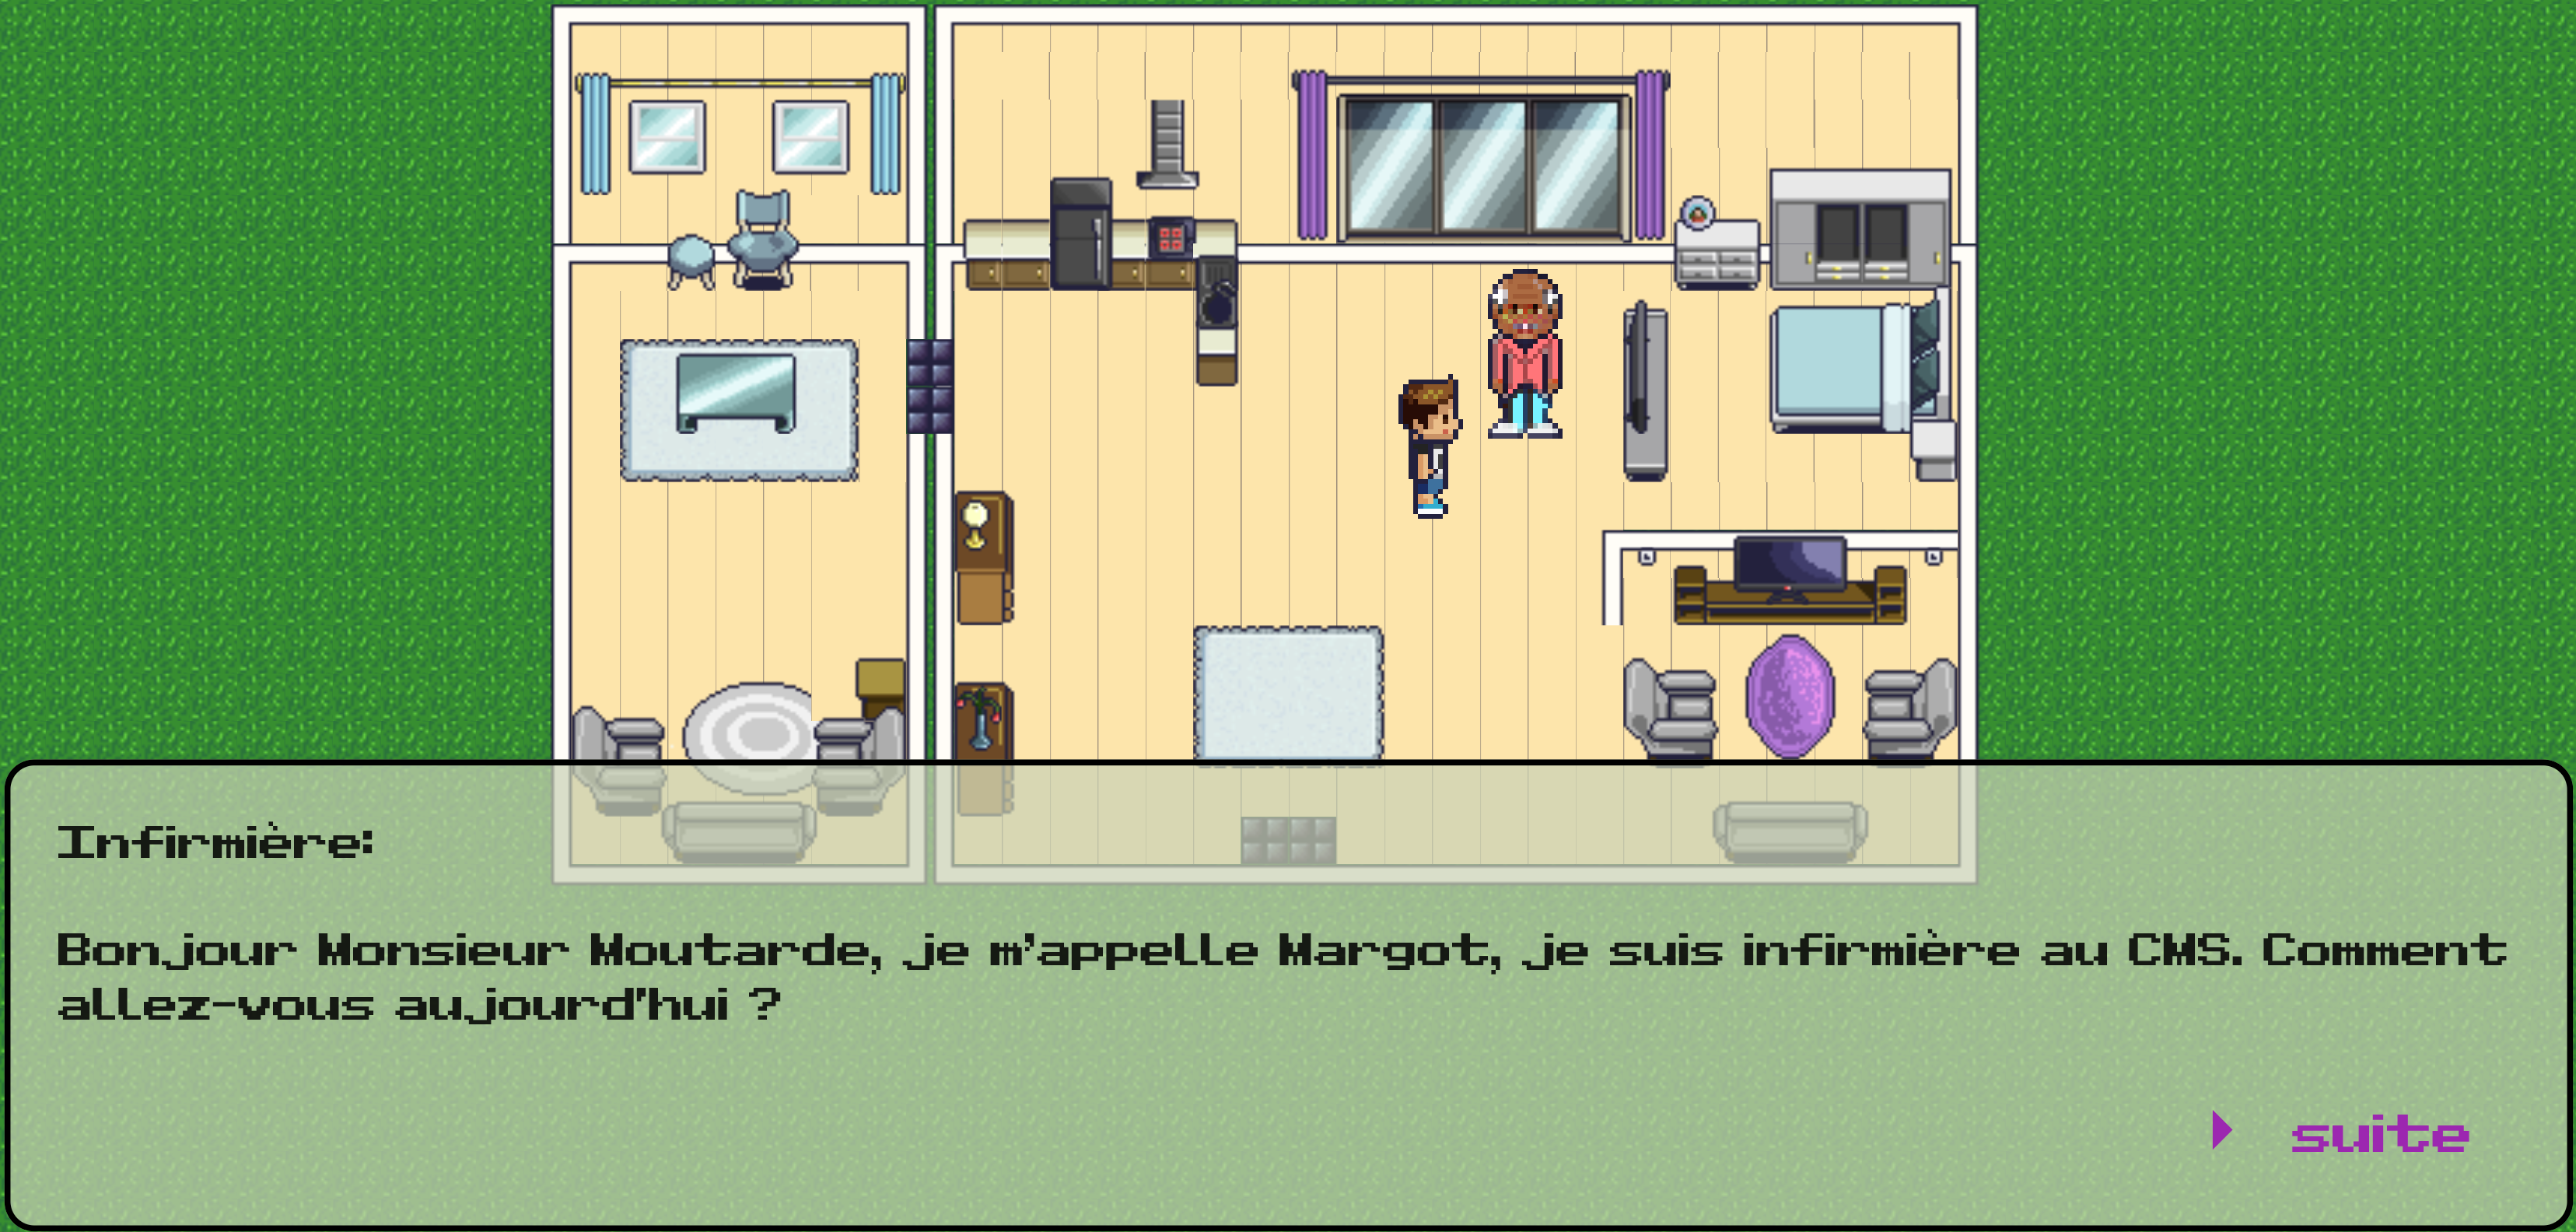
\includegraphics[width=0.8\textwidth ]{images/dialogs/dialog.png}
    \caption{Dialogue}
    \label{fig:pic_dessus}
\end{figure}

Certaines interactions peuvent demander une interaction de l'utilisateur. Si l'utilisateur réagit correctement, il peut gagner des points et bien sûr, s'il réagit de la mauvaise des manières, il en perd. La plupart du temps, en cas de mauvaise réponse, le joueur a le possibilité d'en choisir une autre sans qu'elle ne lui fasse perdre ou gagner d'autres points.

Voici les différents types de dialogue utilisés :
\begin{figure}[H]
    \centering
    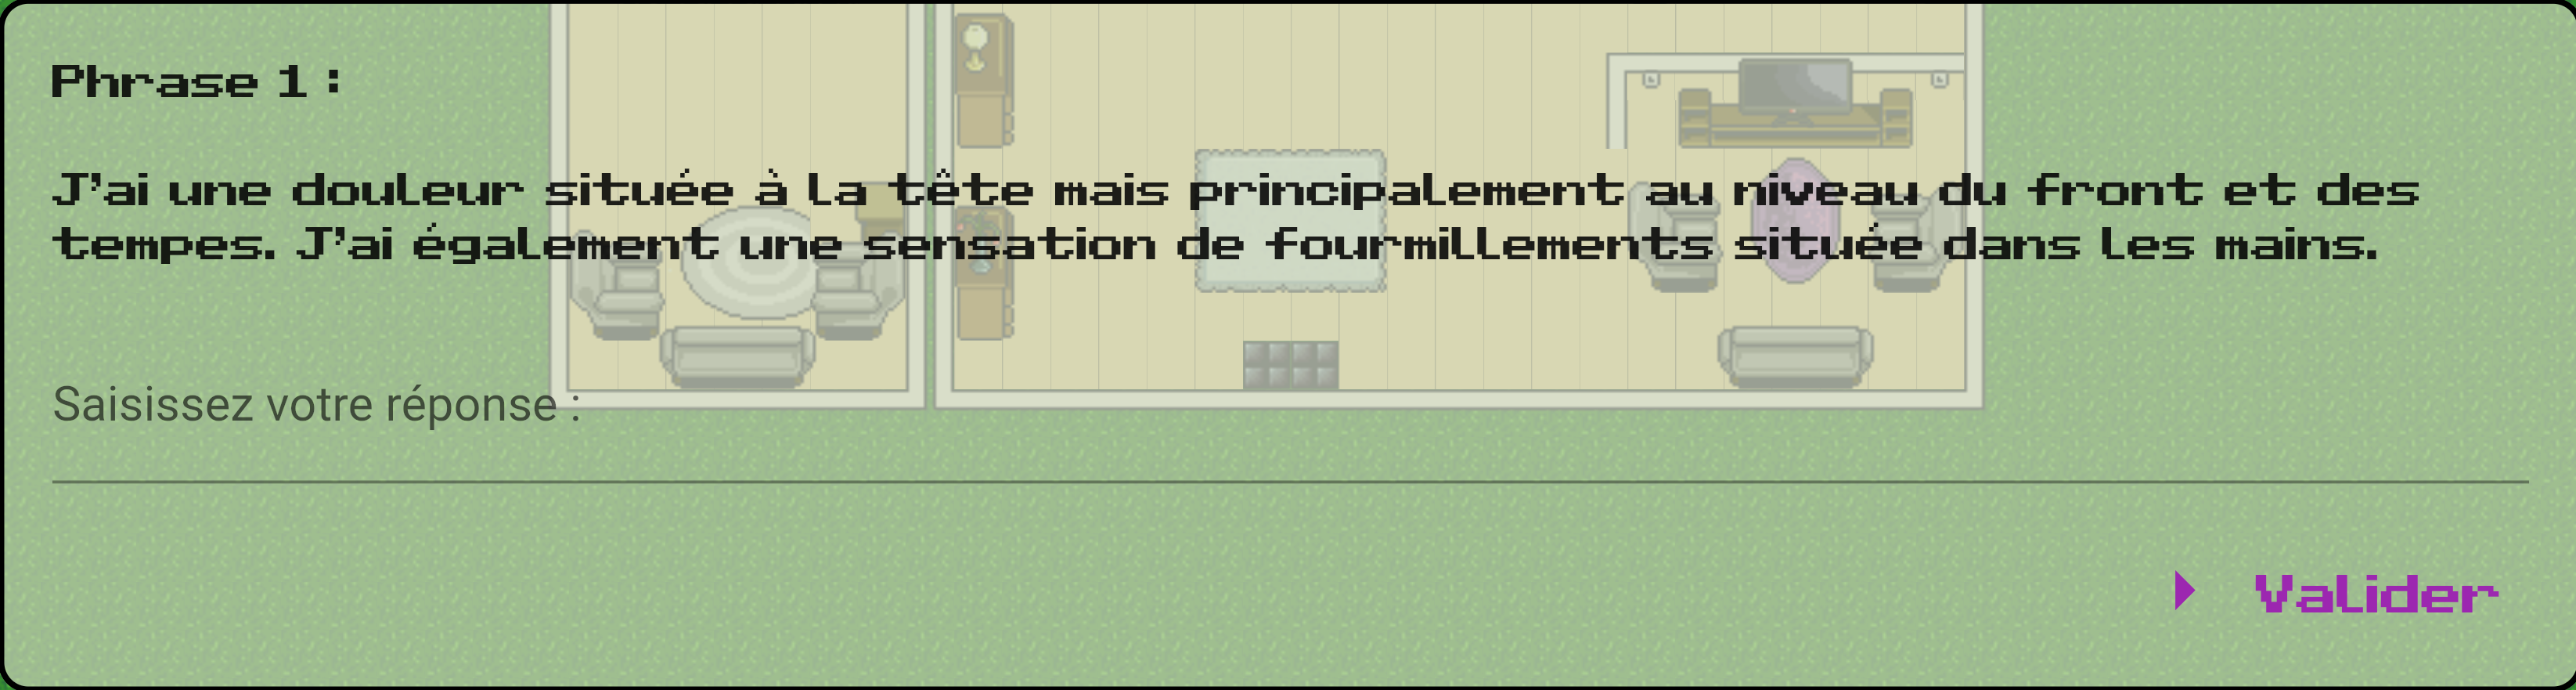
\includegraphics[width=0.8\textwidth ]{images/dialogs/dialogInput.png}
    \caption{Dialogue - Réponse libre}
    \label{fig:pic_dessus}
\end{figure}

\begin{figure}[H]
    \centering
    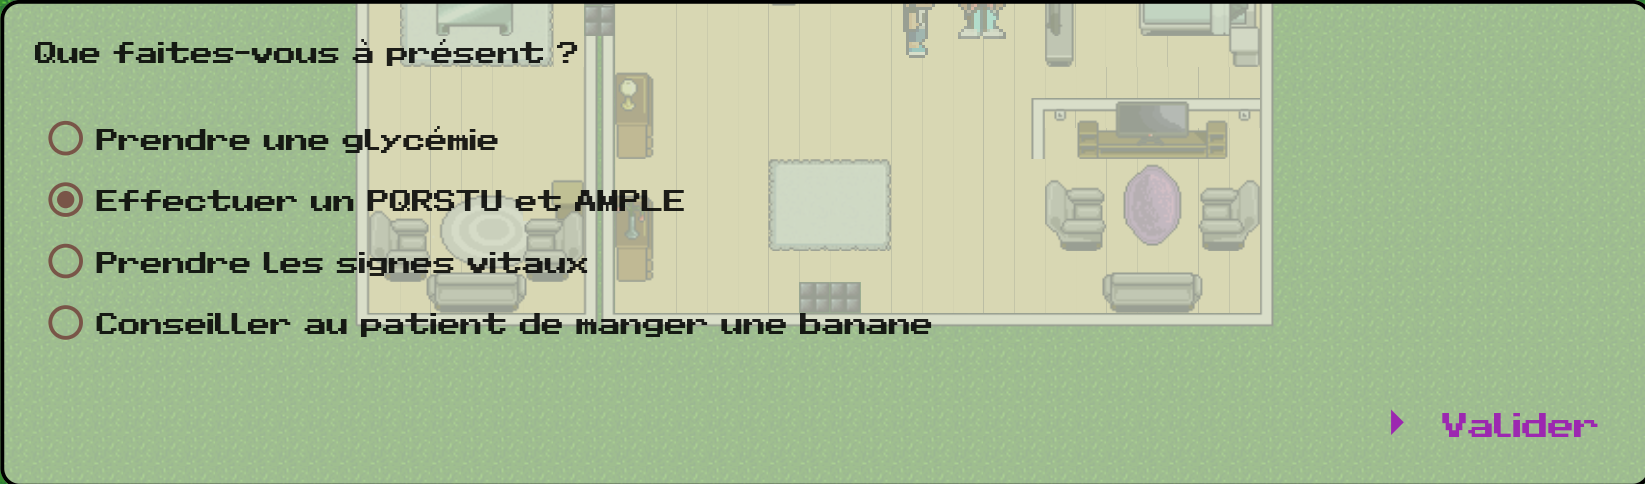
\includegraphics[width=0.8\textwidth ]{images/dialogs/dialogRadioButton.png}
    \caption{Dialogue - Choix unique}
    \label{fig:pic_dessus}
\end{figure}

\begin{figure}[H]
    \centering
    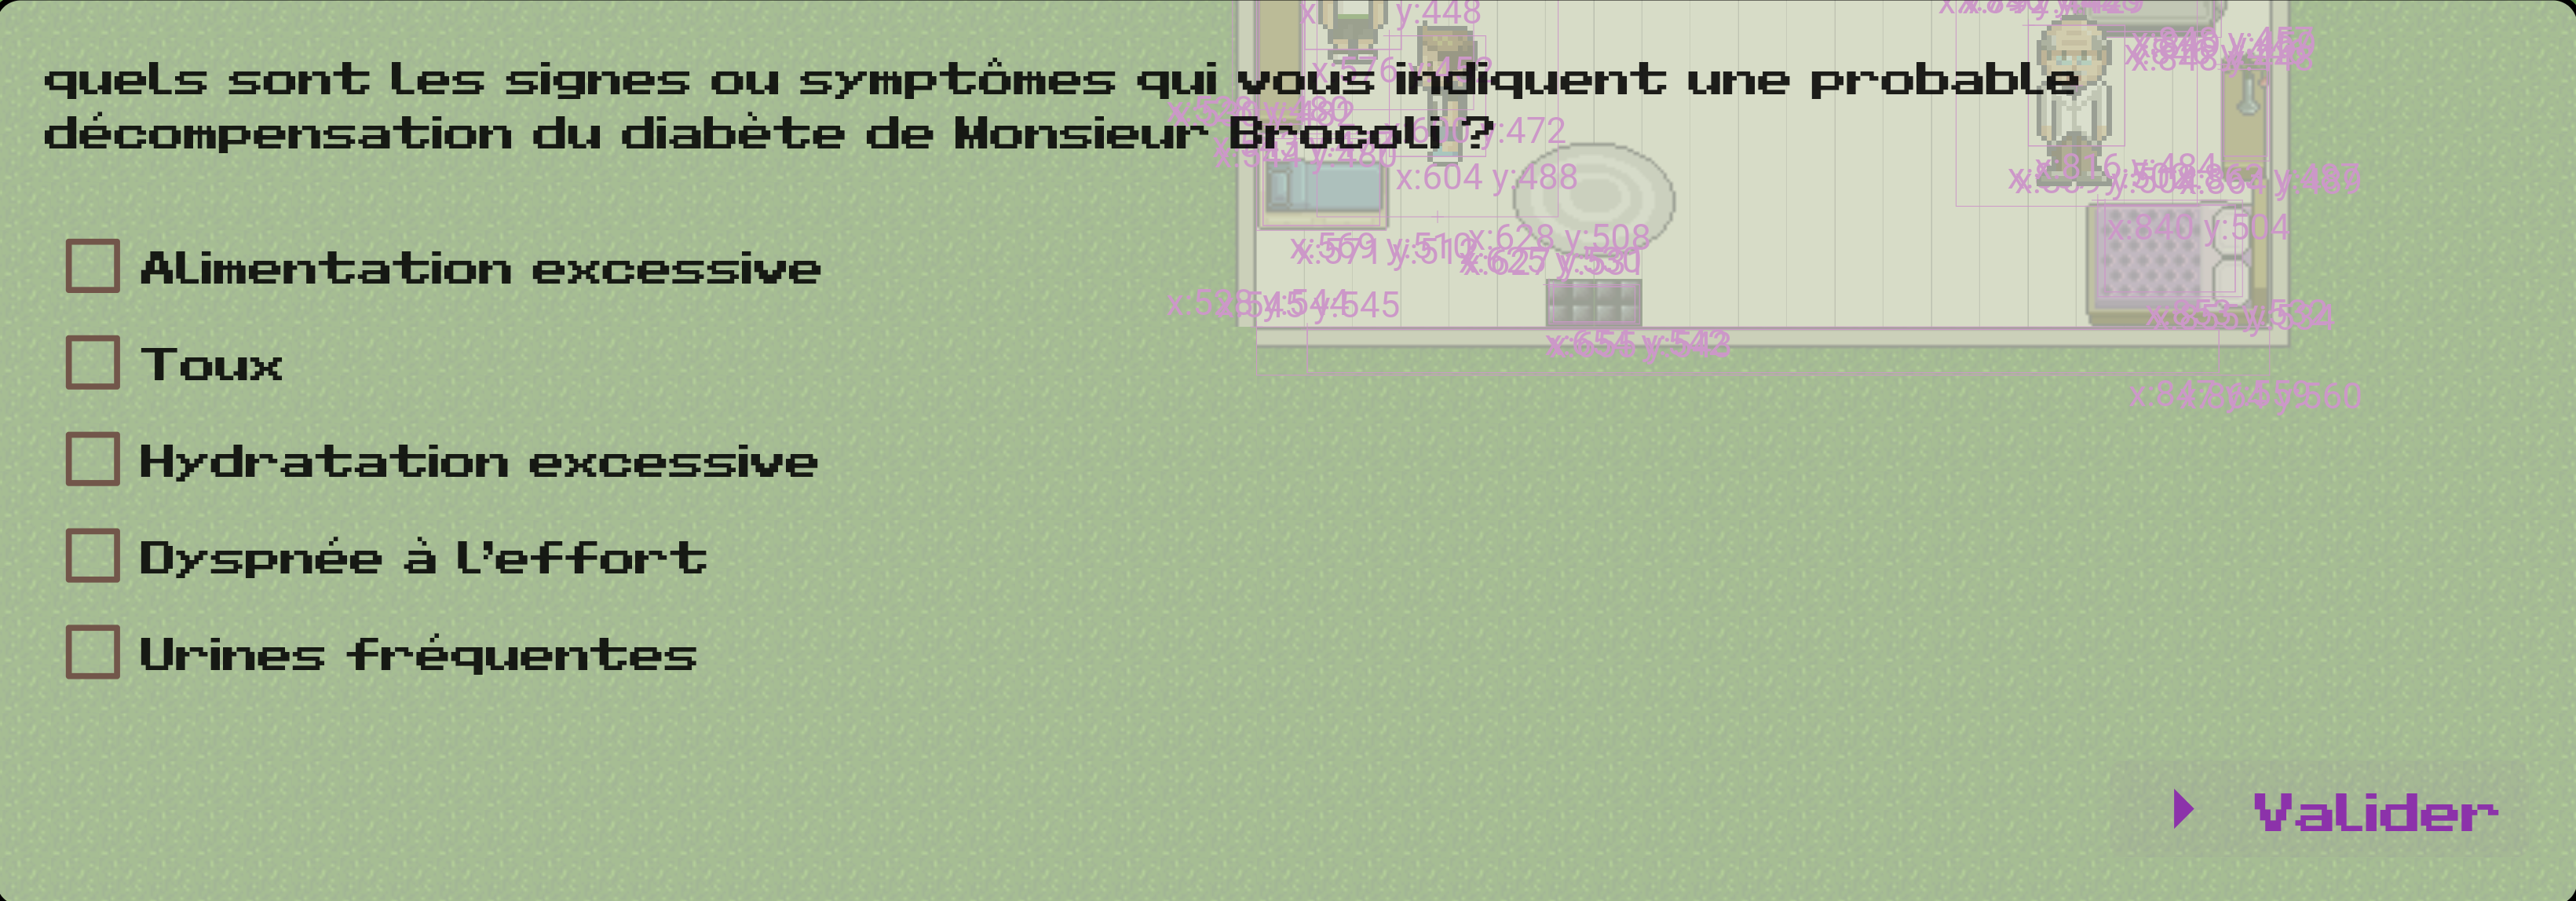
\includegraphics[width=0.8\textwidth ]{images/dialogs/dialogCheckbox.png}
    \caption{Dialogue - Choix multiple}
    \label{fig:pic_dessus}
\end{figure}
